\documentclass[10pt]{article}
\usepackage[ruled, linesnumbered]{algorithm2e}
\usepackage{Jan1, epsfig, subfigure, amssymb, multirow, algorithmic,amsmath}
\usepackage{latexsym,amssymb,epsfig,graphicx,subfigure,rotating,multirow,colortbl,xcolor,amsmath,algorithmic,booktabs,url}
\usepackage{accents}
\usepackage{subfig}
\textwidth 160mm
\textheight 225mm
\voffset 1mm
\oddsidemargin 1mm
\evensidemargin 1mm
\newtheorem{definition}{Definition}
\newtheorem{theorem}{Theorem}
\newtheorem{proposition}{Proposition}
\newtheorem{conjecture}{Conjecture}
\newtheorem{corollary}{Corollary}
\newtheorem{lemma}{Lemma}
\newtheorem{example}{Example}


\usepackage[english]{babel}
\usepackage{blindtext}


\title{Comparison of model simulations}

\author{Anton de Villiers\thanks{HealthQ Technologies, Office 9, First Floor, The Woodmill Lifestyle, Vredenburg Road, Devon Valley,
Stellenbosch, 7600, South Africa}}

\renewcommand{\thefigure}{\arabic{section}.\arabic{figure}}
\renewcommand{\thetable}{\arabic{section}.\arabic{table}}
\begin{document}
\setcounter{page}{1}



\newcommand{\blokkie}{\hspace{.07cm}\Box\hspace{.07cm}}

%%%%% Set up the coloured tables %%%%%
\colorlet{tableheadcolor}{gray!25} % Table header colour = 25% gray
\colorlet{tablerowcolor}{gray!10} % Table row separator colour = 10% gray
\newcommand{\headcol}{\rowcolor{tableheadcolor}}
\newcommand{\rowcol}{\rowcolor{tablerowcolor}}

% The top-most line of a table
\newcommand{\topline}{\arrayrulecolor{black}\specialrule{0.1em}{\abovetopsep}{0pt}%
	\arrayrulecolor{tableheadcolor}\specialrule{\belowrulesep}{0pt}{0pt}%
	\arrayrulecolor{black}}

	% The top-most line of a table
\newcommand{\toplinee}{\arrayrulecolor{black}\specialrule{0.1em}{\abovetopsep}{0pt}%
	\arrayrulecolor{tablerowcolor}\specialrule{\belowrulesep}{0pt}{0pt}%
	\arrayrulecolor{black}}

% The line between the headings and the table body
\newcommand{\midline}{\arrayrulecolor{tableheadcolor}\specialrule{\aboverulesep}{0pt}{0pt}%
	\arrayrulecolor{black}\specialrule{\lightrulewidth}{0pt}{0pt}%
	\arrayrulecolor{white}\specialrule{\belowrulesep}{0pt}{0pt}%
	\arrayrulecolor{black}}

% A line for when the upper row is rowcolor and the next line is white
\newcommand{\midlinecbw}{\arrayrulecolor{tablerowcolor}\specialrule{\aboverulesep}{0pt}{0pt}%
	\arrayrulecolor{black}\specialrule{\lightrulewidth}{0pt}{0pt}%
 	\arrayrulecolor{white}\specialrule{\belowrulesep}{0pt}{0pt}%
	\arrayrulecolor{black}}

% A line with no black, to further separate a rowcolor row and a white row
\newcommand{\midlinecw}{\arrayrulecolor{tablerowcolor}\specialrule{\aboverulesep}{0pt}{0pt}%
	\arrayrulecolor{tablerowcolor}\specialrule{\lightrulewidth}{0pt}{0pt}%
	\arrayrulecolor{white}\specialrule{\belowrulesep}{0pt}{0pt}%
	\arrayrulecolor{black}}

% A line for when the upper row is white and the next line is rowcolor
\newcommand{\midlinewbc}{\arrayrulecolor{white}\specialrule{\aboverulesep}{0pt}{0pt}%
	\arrayrulecolor{black}\specialrule{\lightrulewidth}{0pt}{0pt}%
	\arrayrulecolor{tablerowcolor}\specialrule{\belowrulesep}{0pt}{0pt}%
	\arrayrulecolor{black}}

% sadfsdfsdf sdfsdfsdf
\newcommand{\midlinehr}{\arrayrulecolor{tablerowcolor}\specialrule{\aboverulesep}{0pt}{0pt}%
	\arrayrulecolor{black}\specialrule{\lightrulewidth}{0pt}{0pt}%
	\arrayrulecolor{tableheadcolor}\specialrule{\belowrulesep}{0pt}{0pt}%
	\arrayrulecolor{tablerowcolor}}


% A line for the bottom of the table, when the last row is white
\newcommand{\bottomline}{\arrayrulecolor{white}\specialrule{\aboverulesep}{0pt}{0pt}%
	\arrayrulecolor{black}\specialrule{\heavyrulewidth}{0pt}{\belowbottomsep}}%

% A line for the bottom of the table, when the last row is rowcolor
\newcommand{\bottomlinec}{\arrayrulecolor{tablerowcolor}\specialrule{\aboverulesep}{0pt}{0pt}%
	\arrayrulecolor{black}\specialrule{\heavyrulewidth}{0pt}{\belowbottomsep}}%

\newcommand{\bottomlinect}{\arrayrulecolor{tableheadcolor}\specialrule{\aboverulesep}{0pt}{0pt}%
	\arrayrulecolor{black}\specialrule{\heavyrulewidth}{0pt}{\belowbottomsep}}%
%%%%% Set up the coloured tables %%%%%



\maketitle



\pagestyle{myheadings}


\section{Introduction}

This document contains the most recent results and findings of five distinct complex models programmed in OpenModelica~\cite{OpenModelica}. The models are built to simulate physical complex systems ({\em e.g.}\ systems containing mechanical, electronic, or process-oriented subcomponents) and are described by means of a combination of differential, algebraic and discrete equations where the number of unknowns and the number of equations is identical.

OpenModelica's ``gold-standard'' solver for numerically solving ordinary differential equations (ODEs) is DASSL~\cite{DASSL}. The DASSL solver can simulate all of the models in this document accurately within the OpenModelica framework. In addition to the DASSL solver, numerous other solvers are provided by OpenModelica including Runge-Kutta and Euler based solvers. Finally, OpenModelica also provides a Quantised State Systems (QSS)~\cite{MigoniKofman2009} method, which is still in development. The QSS solvers differs fundamentally from traditional ODE solvers which is based are on the notion of state quantization, ignoring the traditional approach of time discretization when numerically solving ODEs. OpenModelica's version of a QSS solver currently has very limited functionality.

QSS Solver\footnote{QSS Solver is an application that contains a family of QSS implemented solvers for addressing ODE systems.}~\cite{qss} is a modeling and simulation environment for continuous and hybrid systems. This simulation tool describe models using a subset of the Modelica language called MicroModelica~\cite{micro}. QSS Solver supports the entire family of QSS related solvers, including a family of Linearly Implicit QSS (LIQSS)~\cite{MigoniKofman2009} solvers which were created to deal with stiff mathematical systems. The LIQSS solvers may be considered to be more comprehensive solvers than that of the normal QSS methods. In order to convert Modelica models to MicroModelica models, ModelicaCC~\cite{ModelicaCC} is used which consists of four conversion stages. ModelicaCC has four steps to convert models from Modelica syntax to MicroModelica syntax. These steps are:
\begin{itemize}
 \item flatter
 \item antialias
 \item mmo
 \item causalize
\end{itemize}


HealthQ has undertaken to incorporate a QSS solver as well as a first order LIQSS solver in OpenModelica. These solvers aim to build on the current implementation details of the current QSS solver in OpenModelica.

\section{The five models}

Numerical results of five distinct models will be considered in this document. These five models are:
\begin{itemize}
 \item A stiff mathematical ODE system (Stiff)
 \item A pulse model of the tactile arterial palpation of the heartbeat (Pulse)
 \item An ideal diode system in a circuit (Ideal)
 \item A ball bouncing down stairs (BBall)
 \item A simple cardiovascular system (CardioV)
\end{itemize}

\section{The solvers}

All the solvers used have been mentioned in \S1 of this document. These solvers include:
\begin{itemize}
 \item OpenModelica DASSL ({\sf OM\_DASSL})
 \item OpenModelica QSS ({\sf OM\_QSS})
 \item QSS Solver's LIQSS solvers. This includes the first-, second- and third-order LIQSS solvers ({\sf QSS\_LI1}, {\sf QSS\_LI2} \& {\sf QSS\_LI3})
 \item HealthQ's implementation of QSS and LIQSS in OpenModelica ({\sf HQ\_QSS} \& {\sf HQ\_LI})
\end{itemize}

\section{Simulation details}

For each simulation run, the following will be specified:
\begin{itemize}
 \item duration of the simulation,
 \item some key state variables that will be investigated,
 \item the actual completion time of the simulation (including the compilation times, back-end calculations {\em etc.}), and
 \item a conclusion of the obtained results.
\end{itemize}

For the DASSL solver in OpenModelica a tolerance of {\tt{1e-6}} is used and the number of intervals will be fixed at $1\,000$ for all simulations.

In QSS Solver and absolute tolerance of {\tt{1e-6}} and relative tolerance of {\tt{1e-3}} is used.

HealthQ's QSS and LIQSS solver in OpenModelica both  have $\Delta Q_i = 0.001$ for each state variable $i$. This is constant for all models, except the Cardiovascular Circulation model and the Bouncing Ball models where $\Delta Q_i=0.01$. For the Cardiovascular Circulation model the $\Delta Q_i$ is furthermore multiplied by a ``nominal'' value\footnote{This ``nominal'' value is calculated as an approximate average value of the state variable. To retrieve this average value a simulation is run using OpenModelica's DASSL solver. The numerical results are then aggregated for each state variable individually. This average value is then multiplied by the tolerance to provide and adequate step size for the LIQSS solver between any two time steps --- this is done for each state variable.} of each state variable.

\section{Results}

The numerical results and related finding will be considered in this section. The computational times reported are in seconds and are the sum of the {\tt{user}} time and {\tt{sys}} time provided by the UNIX {\tt{time}} command, which is used in conjunction with the executable that is built for each model. The {\tt{user}} time is defined as the {\em total number of CPU-seconds that the process used directly (in user mode) in seconds}, while the {\tt{sys}} time is the {\em total number of CPU-seconds used by the system on behalf of the process (in kernel mode), in seconds}. The total time {\tt{user}}$+${\tt{sys}} indicates the total amount of actual CPU time a simulation uses.

\subsection{A stiff mathematical system}

The first model is a simple ODE system that is mathematically stiff. The model is:
\begin{eqnarray*}
 \dot{x}_1(t) &=& 0.01x_2(t)\\
 \dot{x}_2(t)& = &-100x_1(t) -100x_2(t) +2020
\end{eqnarray*}
with initial solutions $x_1(0) =0$ and $x_2(0)=20$.

This first model was specifically chosen to highlight the consistency between solvers (and their applications) when a model is simulated correctly. The results are shown in Table~\ref{Tab1}. The simulation was run for 500 seconds in total. In this case both the state variables $x_1(t)$ and $x_2(t)$ are considered in particular. In this case all the solvers were able to solve the model and the numerical results were very much similar, except for the QSS solvers (not the linearly implicit versions). Figure~\ref{Fig1} displays some graphical results of this model.

\begin{table}[htbp]
	\centering\footnotesize
		\begin{tabular}{ccccccccc}
    \topline	\headcol
    Solver&&\sf{OM\_DASSL}& \sf{OM\_QSS}& \sf{QSS\_LI1}& \sf{QSS\_LI2}&\sf{QSS\_LI3}& \sf{HQ\_QSS}& \sf{HQ\_LI}\\\midline
    Sim Time&& 0.009&2.521&0.256&0.027&0.008&0.109&0.014\\\bottomline
    \end{tabular}\vspace{-0.1cm}
\caption{Simulation times of Stiff.}
\label{Tab1}
    \end{table}

    \begin{figure}[htbp]
\begin{center}
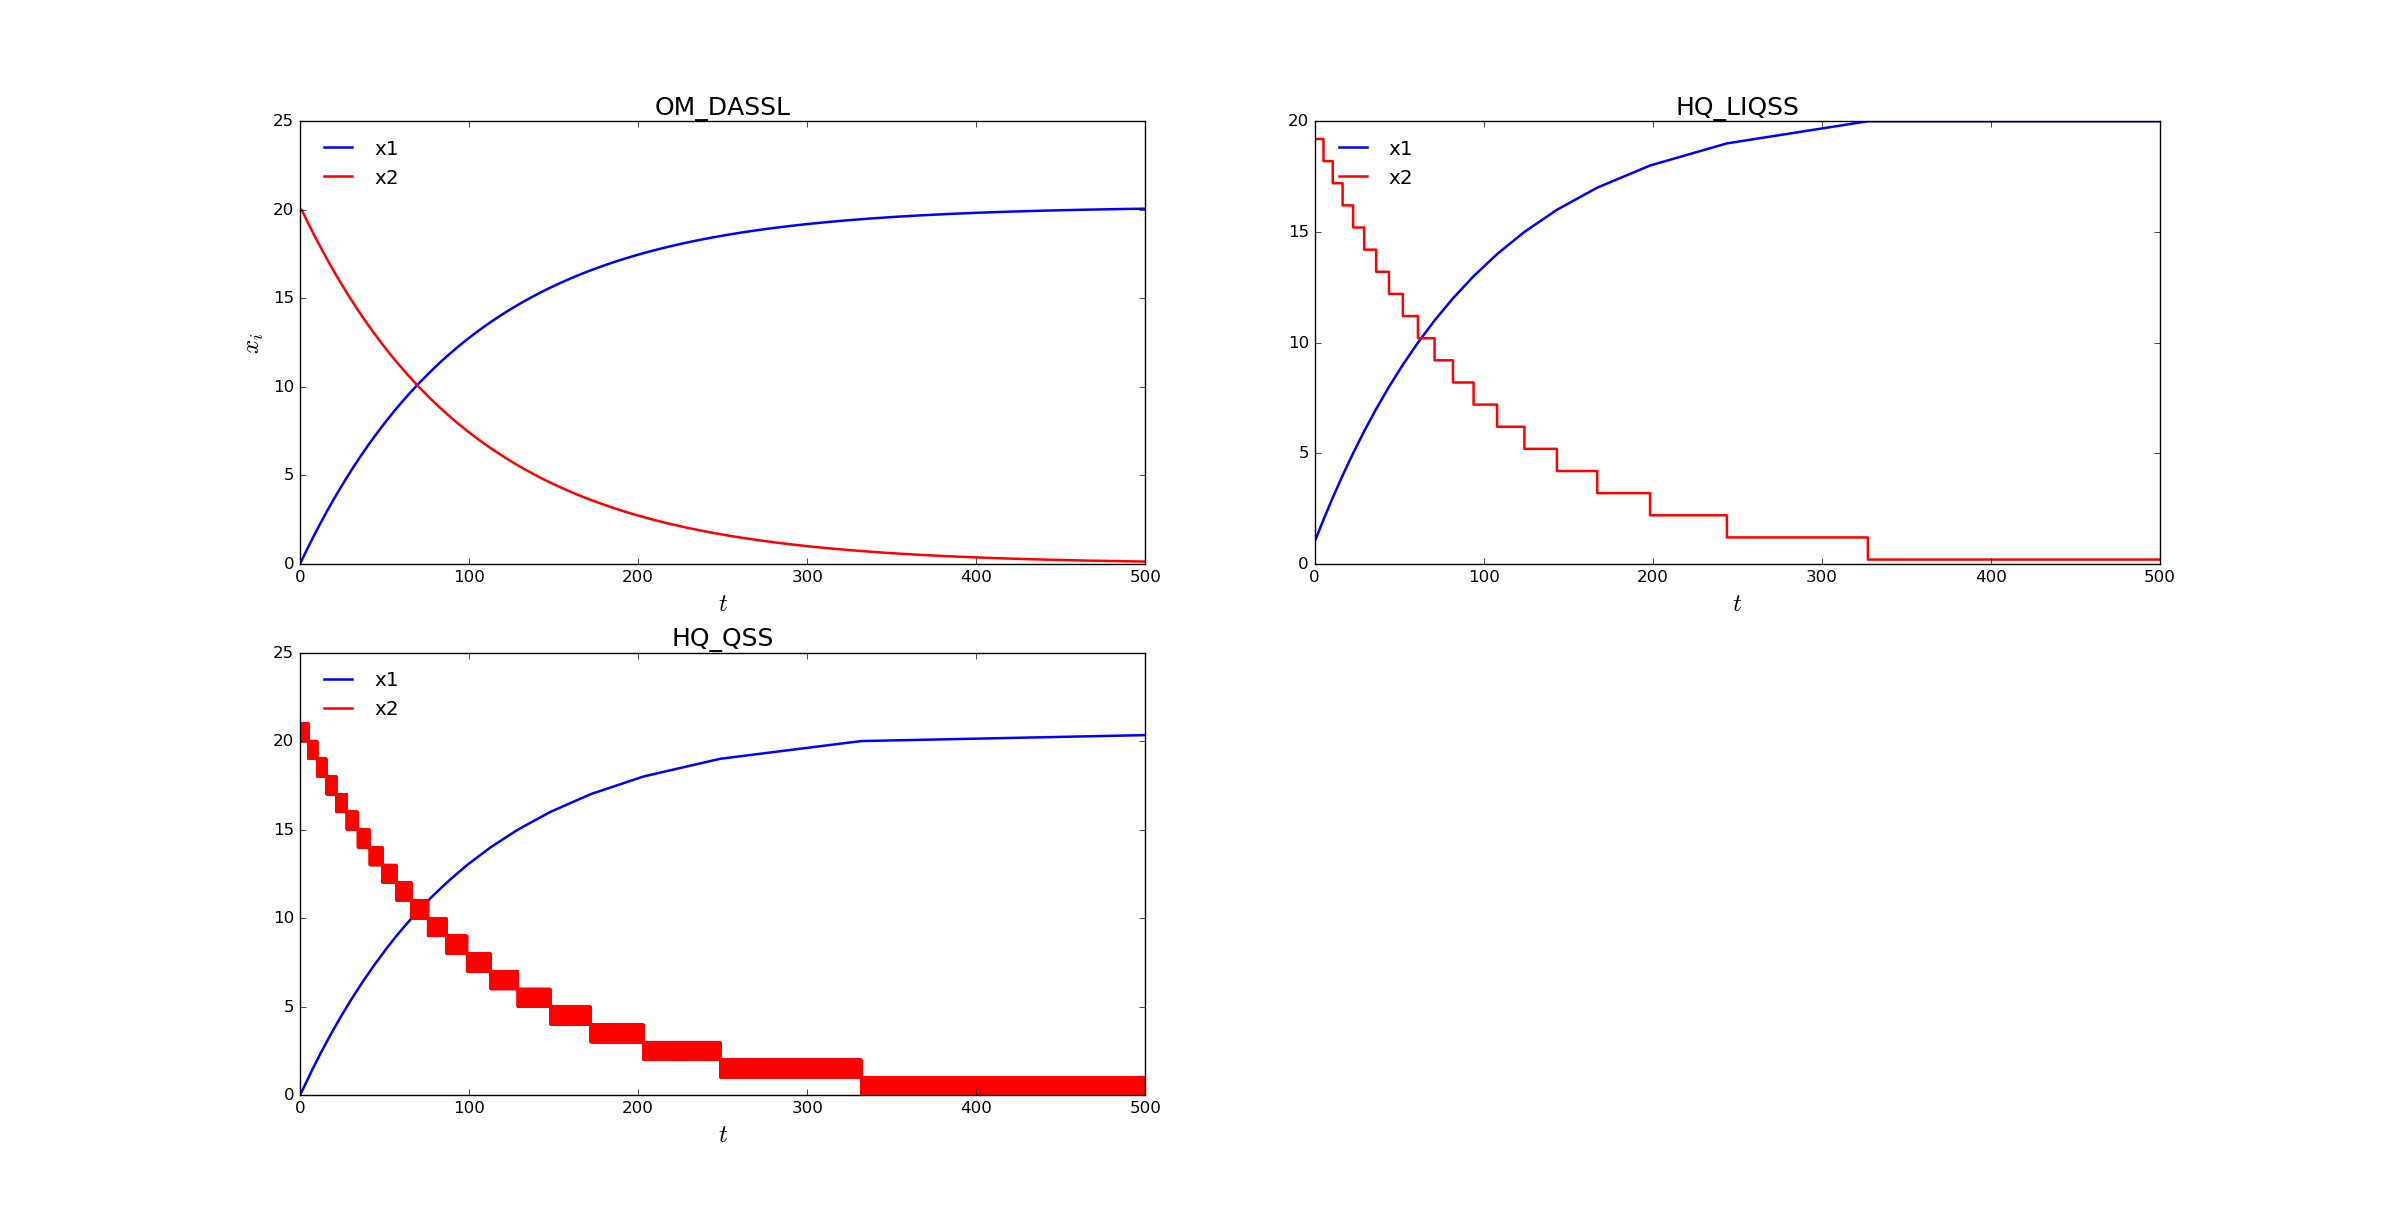
\includegraphics[scale=0.32, clip,trim={55mm 15mm 55mm 20mm}]{./Figures/Model1.png}
\end{center}
\vspace{-0.5cm}
\caption{Simulation results of Stiff for the first 500 seconds of the simulation runs for (a) {\sf{OM\_DASSL}}, (b) {\sf{HQ\_LIQSS}} and (c) {\sf{HQ\_QSS}} with large quantums in (b) and (c). These artificially large quantums in {\sf{HQ\_LIQSS}} and   {\sf{HQ\_QSS}} were not used in the actual simulations --- it is merely for illustration purposes.}\label{Fig1}
\end{figure}

\newpage

\phantom{2}

\newpage

\subsection{Pulse}

The Pulse model simulates a pulse or heartbeat of a human. This model contains an event which changes by means of sinus oscillation -- that is, the pulse is quicker when the sinus value is larger than zero and the oscillations are slower when the sinus value is less than zero. Simulation were performed for 100 seconds. It was a difficult task to convert the Pulse model to simulate successfully in QSS Solver, but it was eventually possible by creating a piecewise function in QSS Solver. The model therefore had to be adjusted for the QSS Solver application. In this case the {\tt{phi}} variable is of importance and will be considered in the results.

Table~\ref{Tab2} contains the simulation times of this model. Two solvers encountered problems with this model, those being {\sf{OM\_QSS}} and {\sf{QSS\_LI1}}. The remainder of the solvers had no problems simulating the model. Figure~\ref{Fig2} shows how the {\sf{OM\_DASSL}} and {\sf{QSS\_LI3}} solvers addressed the model and provides similar solutions.

\begin{table}[htbp]
	\centering\footnotesize
		\begin{tabular}{ccp{8cm}}
    \topline	\headcol
    Solver&Sim time& Comments\\\midline
     \sf{OM\_DASSL}& 0.058&Correct simulation results obtained\\\rowcol
     \sf{OM\_QSS}& 8.950$^*$& Only 1 second simulation time\\
     \sf{QSS\_LI1}&N/A& Unable to solve model. QSS Solver crashes\\\rowcol
     \sf{QSS\_LI2}&0.001& Correct simulation results obtained \\
     \sf{QSS\_LI3}&0.070& Correct simulation results obtained \\\rowcol
     \sf{HQ\_QSS}& 0.189& Correct simulation results obtained\\
     \sf{HQ\_LI}& 0.675&Correct simulation results obtained\\\bottomline
    \end{tabular}
\caption{Simulation results of Pulse.}
\label{Tab2}
    \end{table}

    \begin{figure}[htbp]
\begin{center}
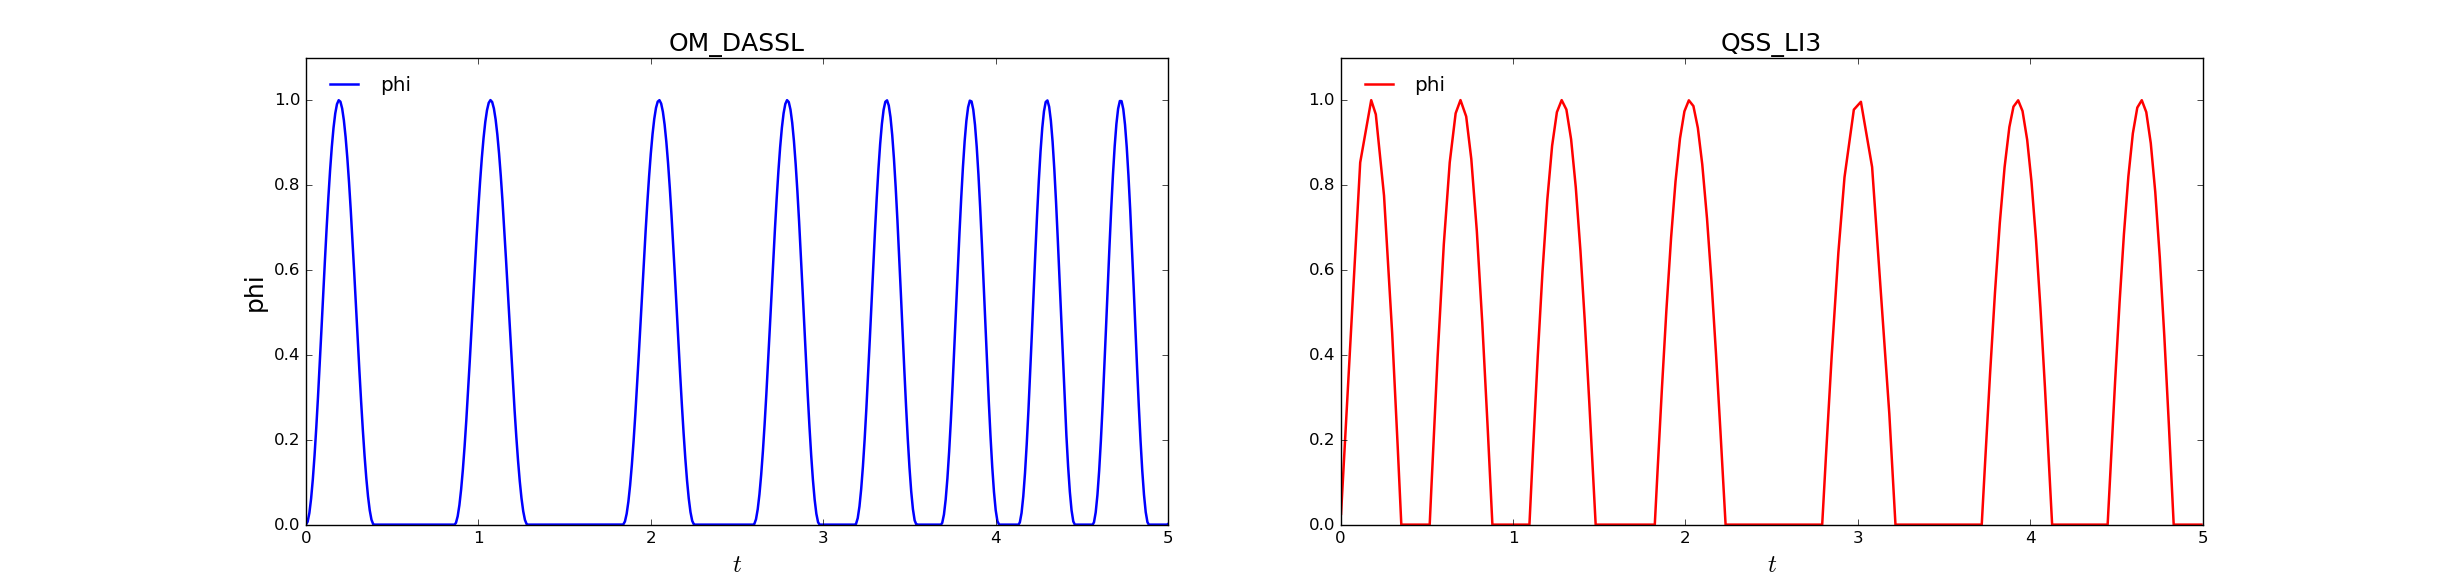
\includegraphics[scale=0.32, clip,trim={55mm 1mm 55mm 0mm}]{./Figures/Model2.png}
\end{center}
\vspace{-0.5cm}
\caption{Simulation results of Pulse for the first 5 seconds of the simulation runs for (a) {\sf{OM\_DASSL}} and (b) {\sf{QSS\_LI3}}.}\label{Fig2}
\end{figure}

\newpage

\subsection{Ideal diode}

The ideal diode or perfect diode is a two terminal device, which completely allows the electric current without any loss under forward bias and completely blocks the electric current with infinite loss under reverse bias. An ideal diode is a good example as it contains some conditional equations for when the flow is on or off.

\begin{table}[htbp]
	\centering\footnotesize
		\begin{tabular}{ccp{8cm}}
    \topline	\headcol
    Solver&Sim time& Comments\\\midline
     \sf{OM\_DASSL}& 0.205&Correct simulation results obtained\\\rowcol
     \sf{OM\_QSS}& 116.006 &Can only simulate 321 seconds in total.\\
     \sf{QSS\_LI1}&None&No feasible conversion\\\rowcol
     \sf{QSS\_LI2}&None &No feasible conversion \\
     \sf{QSS\_LI3}&None &No feasible conversion \\\rowcol
     \sf{HQ\_QSS}& None&Segmentation fault thrown \\
     \sf{HQ\_LI}& 34.889&Correct simulation results obtained\\\bottomline
    \end{tabular}
\caption{Simulation results of Ideal.}
\label{Tab3}
    \end{table}

This model cannot be reduced to MicroModelica by means of ModelicaCC as the causalize step suggests that the number of variables and equations do not match. Therefore simulation of this model is not possible in QSS Solver.




The simulation time is set at 1\,000 seconds. The {\tt{resistance.q}} variable is considered in this model as a key variable. Table~\ref{Tab3} contains a summary of simulation run results, while Figure~\ref{Fig3} displays the {\sf{OM\_DASSL}} and {\sf{HQ\_LI}} solver results, which were the only two solvers that could solve the model successfully for 1\,000 seconds.


    \begin{figure}[htbp]
\begin{center}
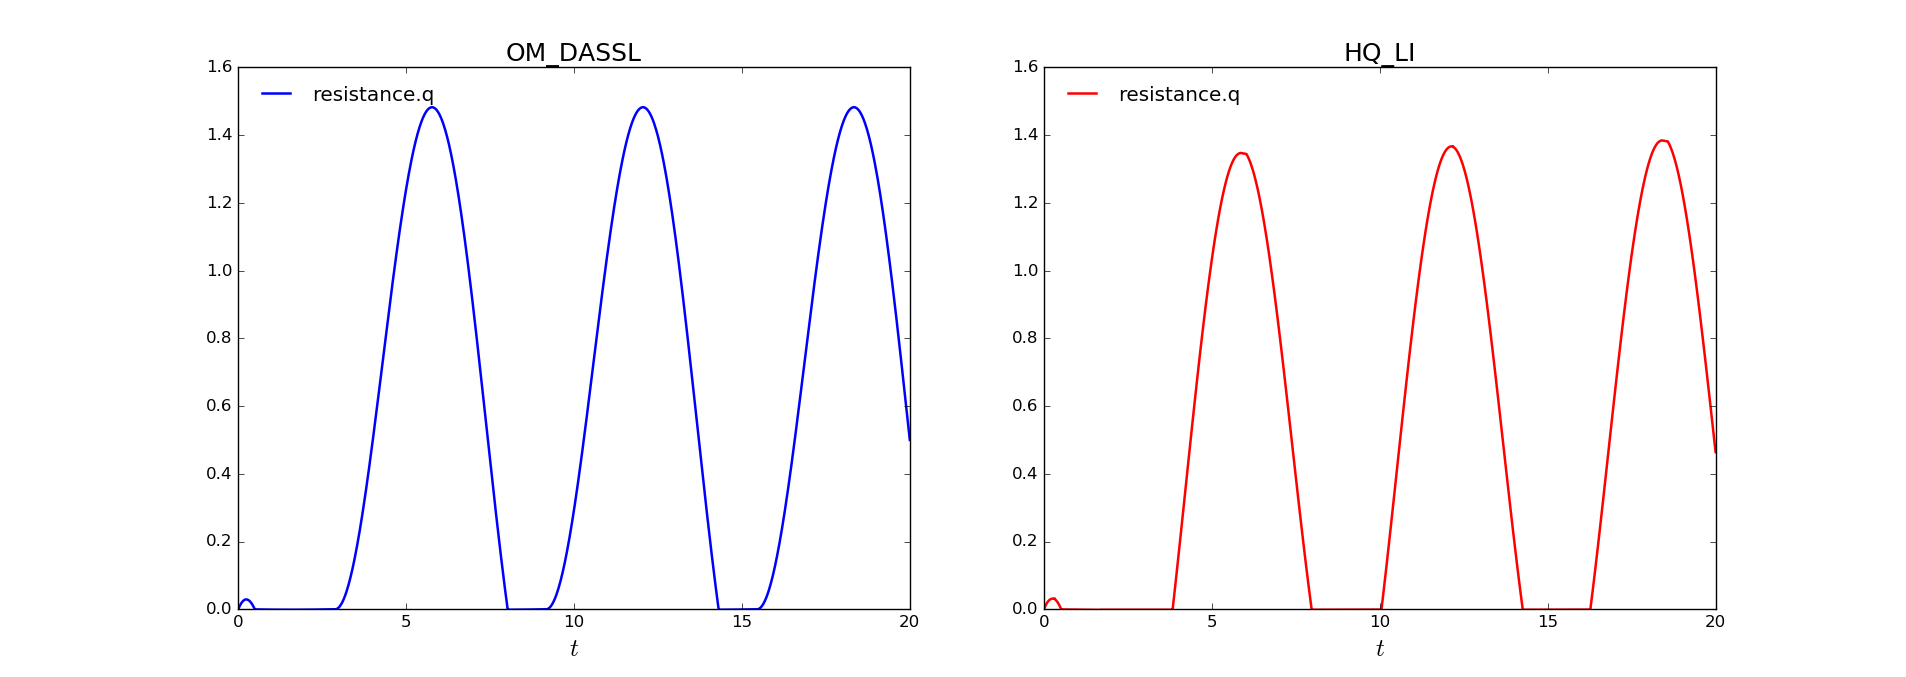
\includegraphics[scale=0.32, clip,trim={50mm 1mm 45mm 10mm}]{./Figures/Model3.png}
\end{center}
\vspace{-0.5cm}
\caption{Simulation results of Ideal for the first 20 seconds of the simulation runs for (a) {\sf{OM\_DASSL}} and (b) {\sf{OM\_LI}}.}\label{Fig3}
\end{figure}

\newpage

\subsection{Bouncing ball}
The bouncing ball is an example of a hybrid system, containing events and conditional expressions. We considered two variations on this model, one where the ball is released in a forward direction and bounces on a flat surface. The alternative model contains stairs and the ball bounces down these stairs.

\subsubsection{Flat surface bouncing}

The model was simulated for 25 seconds in each run. Only the {\sf{OM\_DASSL}} solver was able to successfully solve this model as expected. Table~\ref{Tab41} contains a summary of the simulation runs, while Figure~\ref{Fig41} contains the graphical results for each simulation run. From these results it is clear that the solvers contain fundamental differences, especially with respect to this model.

\begin{table}[htbp]
	\centering\footnotesize
		\begin{tabular}{ccp{8cm}}
    \topline	\headcol
    Solver&Sim time&Comments\\\midline
     \sf{OM\_DASSL}&0.025&Correct simulation results obtained\\\rowcol
     \sf{OM\_QSS}& 141.846&No events are triggered\\
     \sf{QSS\_LI1}&0.259&Ball continually bounces higher\\\rowcol
     \sf{QSS\_LI2}&0.105 &Erratic bouncing \\
     \sf{QSS\_LI3}&0.011&Erratic bouncing \\\rowcol
     \sf{HQ\_QSS}&4.216 &The ball bounces to the same approximate height \\
     \sf{HQ\_LI}& 7.245& The ball does not bounce high enough\\\bottomline
    \end{tabular}
\caption{Simulation results of BBall on a flat surface.}
\label{Tab41}
    \end{table}

        \begin{figure}[htbp]
\begin{center}
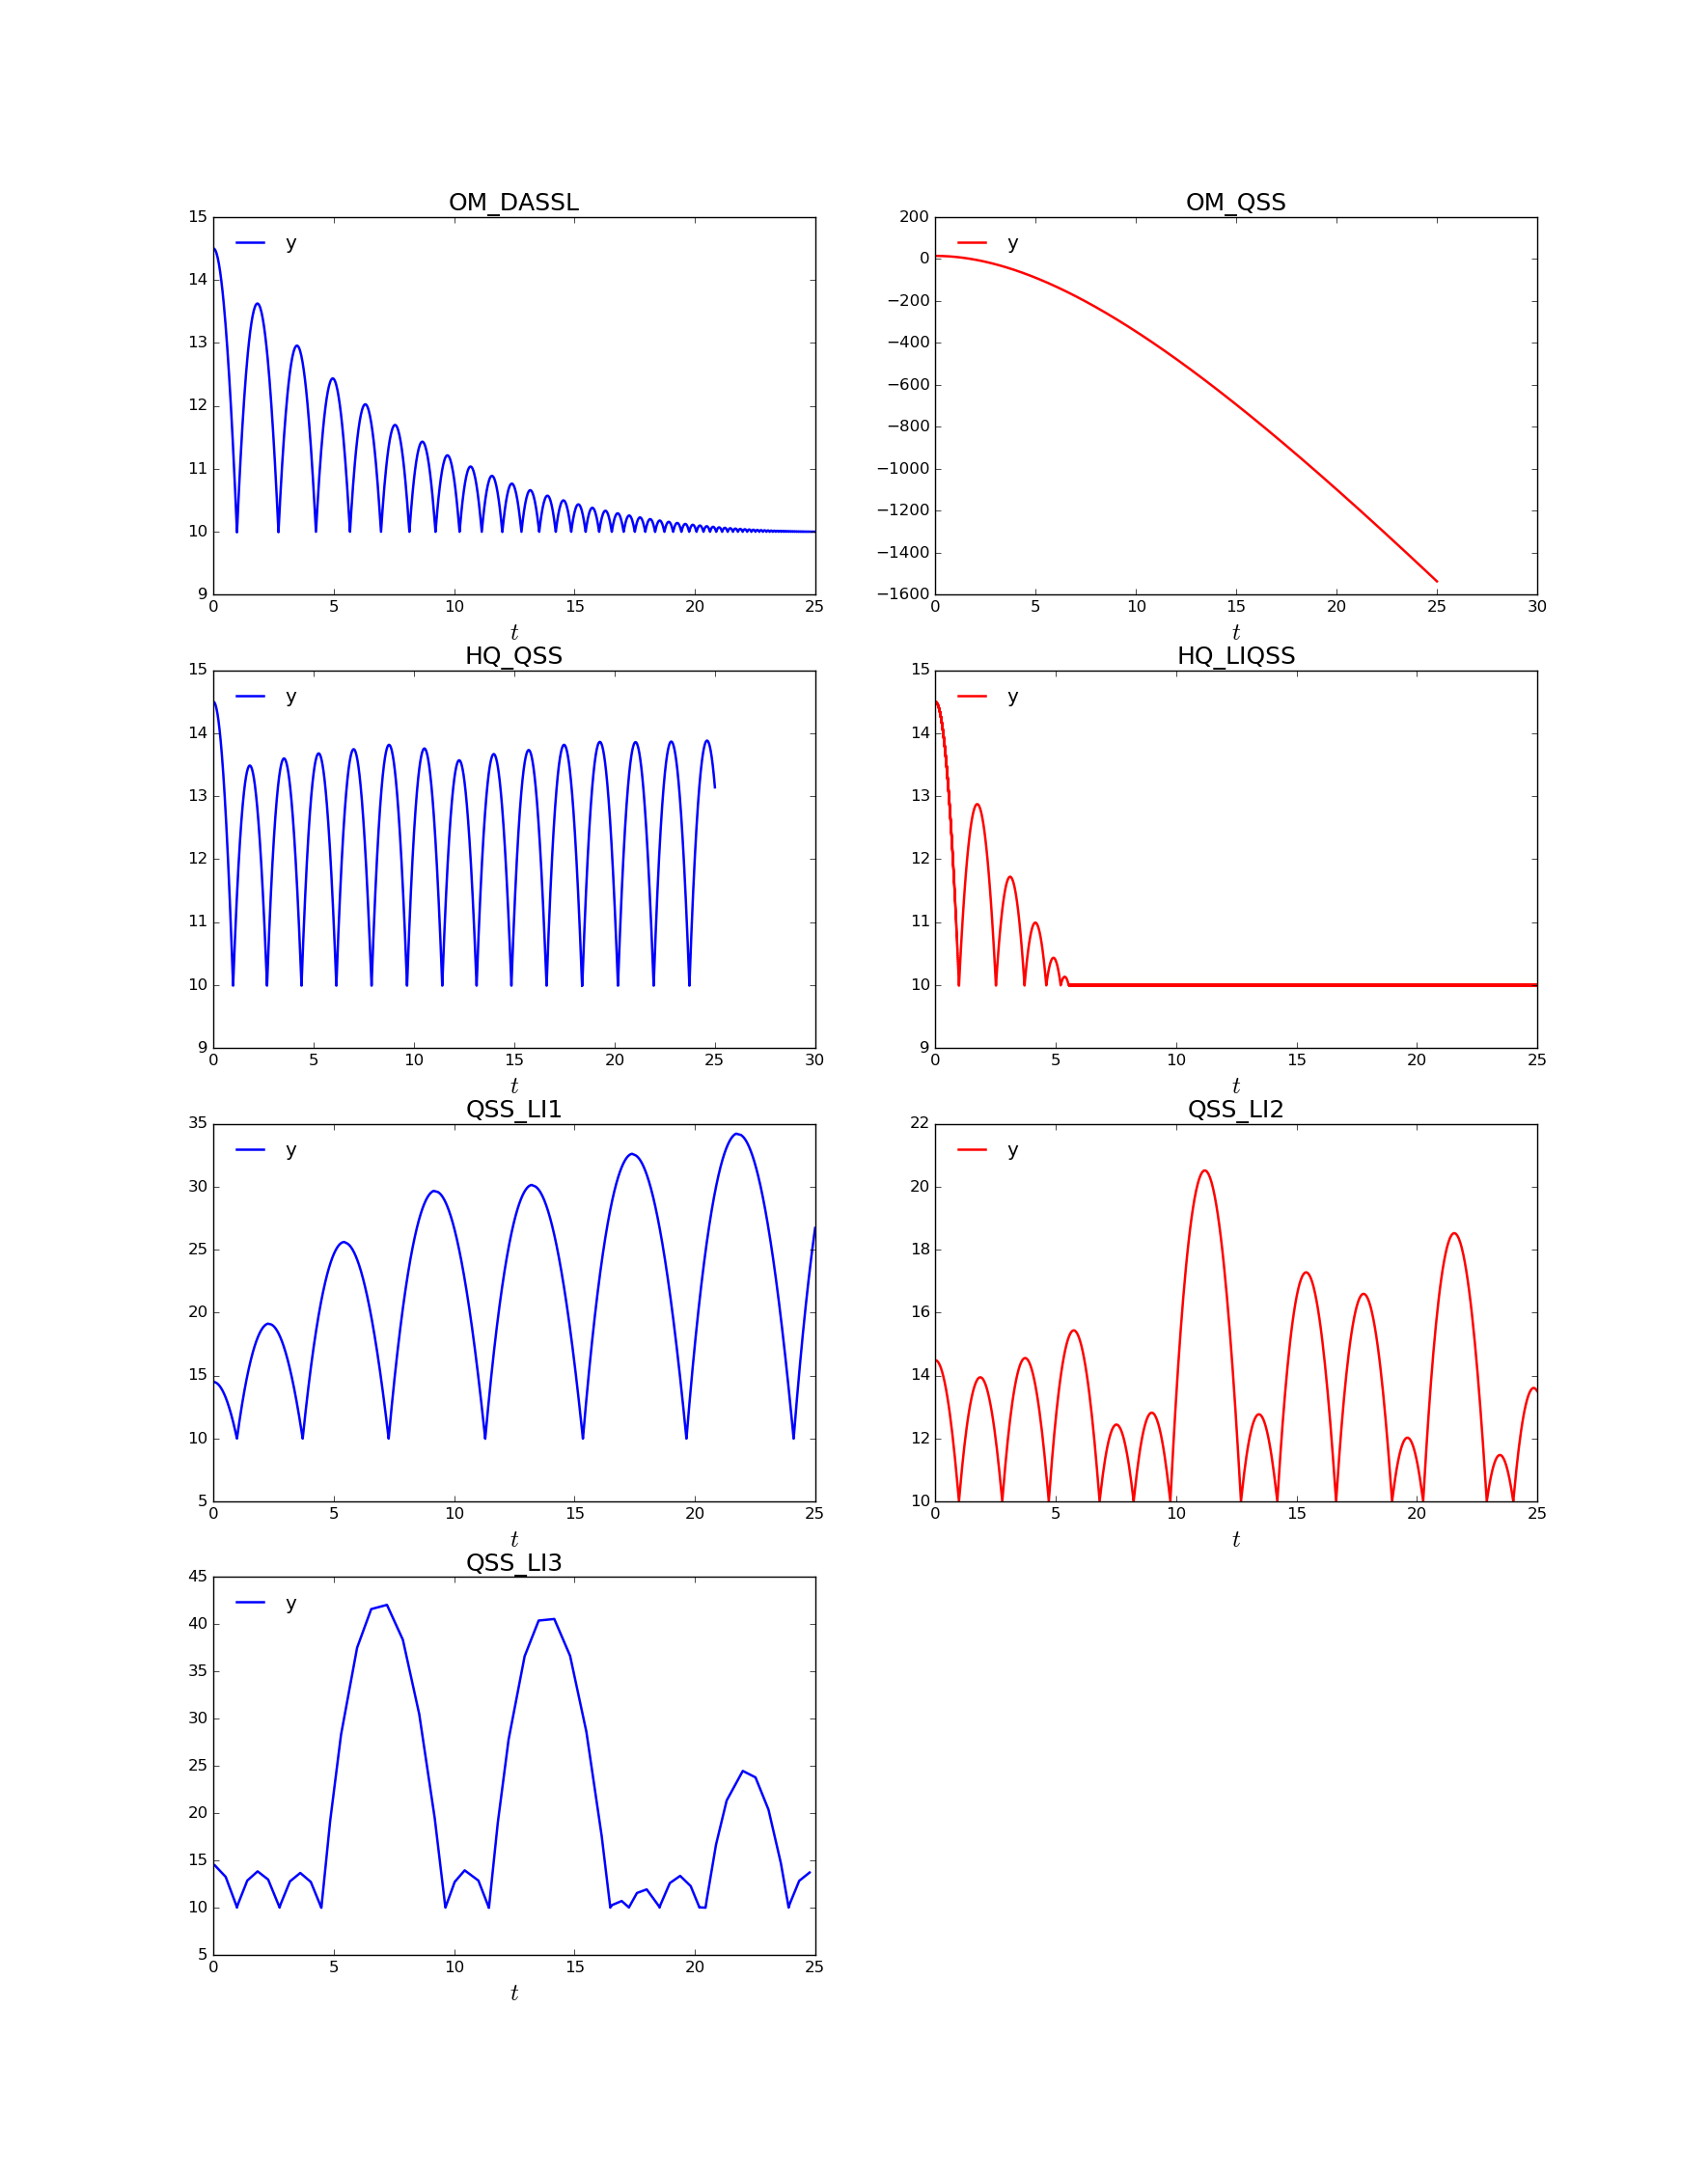
\includegraphics[scale=0.42, clip,trim={40mm 40mm 30mm 40mm}]{./Figures/Model6.png}
\end{center}
\vspace{-0.5cm}
\caption{Simulation results of BBall on a flat surface for (a) {\sf{OM\_DASSL}}, (b) {\sf{OM\_QSS}}, (c) {\sf{HQ\_QSS}}, (d) {\sf{HQ\_LIQSS}},  (e) {\sf{QSS\_LI1}},  (f) {\sf{QSS\_LI2}} and (g) {\sf{QSS\_LI3}}. Only the {\sf{OM\_DASSL}} solver provides the expected and correct simulation results.}\label{Fig41}
\end{figure}

\newpage

\subsubsection{Descending stairs}

This model is further complicated by the addition of adding stairs. The simulation is run for 40 seconds and the important state variables considered are {\tt{y}} and {\tt{stair}}.

This model is particularly difficult to simulate. The only model that was able to simulate this model correct was {\sf{OM\_DASSL}}. All the other solvers had some form of inaccuracies or faults that renders the simulation results as not useful. Table~\ref{Tab42} contains a summary of the simulation runs, while Figure~\ref{Fig42} contains the graphical results

\begin{table}[htbp]
	\centering\footnotesize
		\begin{tabular}{ccp{8cm}}
    \topline	\headcol
    Solver&Sim time&Comments\\\midline
     \sf{OM\_DASSL}&0.017&Correct simulation results obtained.\\\rowcol
     \sf{OM\_QSS}&190.237 &No events are triggered\\
     \sf{QSS\_LI1}&None&QSS Solver crashes\\\rowcol
     \sf{QSS\_LI2}& 0.156&Erratic bouncing\\
     \sf{QSS\_LI3}&0.015&Erratic bouncing \\\rowcol
     \sf{HQ\_QSS}&5.015 & Ball sometimes bounces too high \\
     \sf{HQ\_LI}& 9.514& The ball does not bounce high enough\\\bottomline
    \end{tabular}
\caption{Simulation results of BBall.}
\label{Tab42}
    \end{table}

    \begin{figure}[htbp]
\begin{center}
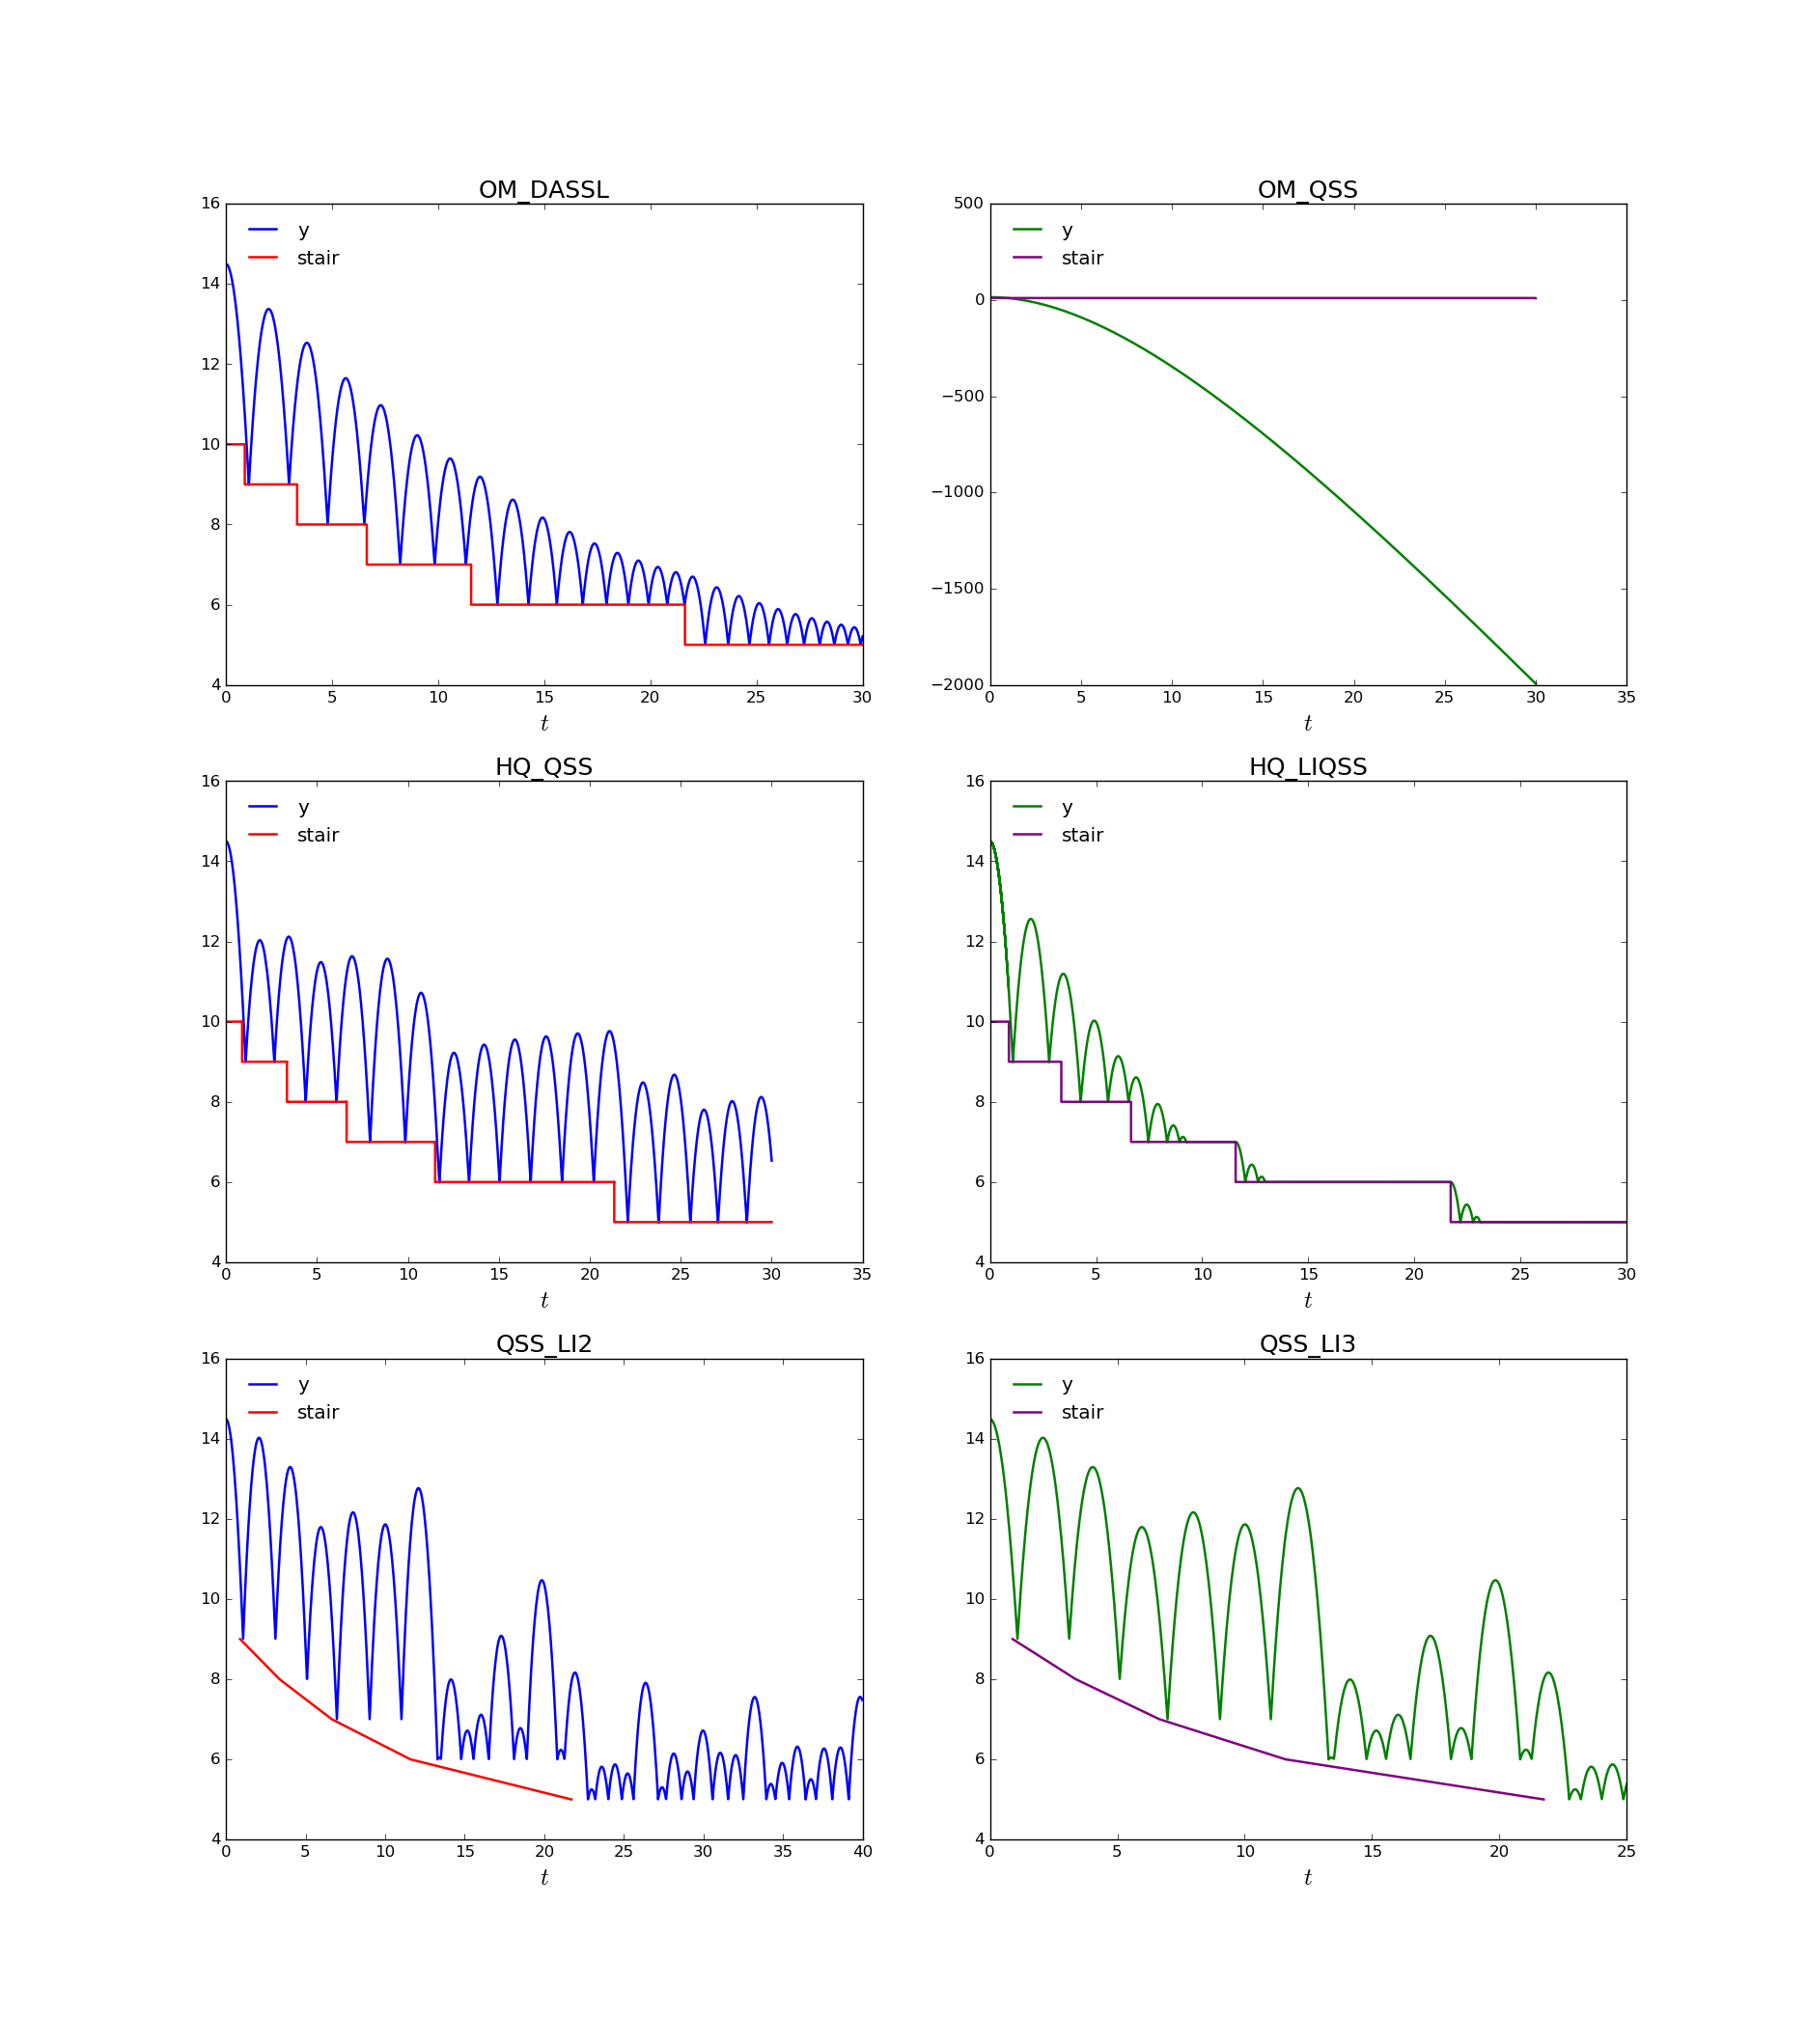
\includegraphics[scale=0.4, clip,trim={45mm 40mm 30mm 40mm}]{./Figures/Model4.png}
\end{center}
\vspace{-0.5cm}
\caption{Simulation results of BBall down a set of stairs for (a) {\sf{OM\_DASSL}}, (b) {\sf{OM\_QSS}}, (c) {\sf{HQ\_QSS}}, (d) {\sf{HQ\_LIQSS}},  (e) {\sf{QSS\_LI2}} and (f) {\sf{QSS\_LI3}}. Only the {\sf{OM\_DASSL}} solver provides the expected and correct simulation results.}\label{Fig42}
\end{figure}

\newpage

\subsection{Cardiovascular Circulation}

The cardiovascular circulation model is a simple system of the cardiovascular system of the human body. This model entails elements from all the other models presented in this document. The simulation time is set at 100 seconds, but only {\sf{OM\_DASSL}} could solve the model successfully for this time period. The {\sf{HQ\_LI}} solver can solve the model for shorter periods of time such as 10 seconds. In this simulation the two state variables that were investigated are {\tt{heart.leftHeart.ventricle.compartment.P}} and {\tt{heart.leftHeart.characteristicResistor.flow\_out.P}}.

Table~\ref{tab5} contains of summary of the simulation runs, while Figure~\ref{Fig5} displays the graphical results of {\sf{OM\_DASSL}} and {\sf{HQ\_LIQSS}} for the first three seconds of a simulation run.

\begin{table}[htbp]
	\centering\footnotesize
		\begin{tabular}{ccp{8cm}}
    \topline	\headcol
    Solver&Sim time& Comments\\\midline
     \sf{OM\_DASSL}& 2.503&Solves the model ideally. \\\rowcol
     \sf{OM\_QSS}& None& Unable to solve the model for more than 0.01 seconds.\\
     \sf{QSS\_LI1}&None & Unable to simulate in the MicroModelica framework.\\\rowcol
     \sf{QSS\_LI2}&None & Unable to simulate in the MicroModelica framework.\\
     \sf{QSS\_LI3}&None & Unable to simulate in the MicroModelica framework.\\\rowcol
     \sf{HQ\_QSS}& None& Unable to simulate the model for more than a second. The model is too stiff and the QSS produces very short increments in time steps.\\
     \sf{HQ\_LI}& 117.846$^*$&Slow simulation speed. Cannot simulate the full 100 seconds as too many time steps are created and the memory becomes overloaded. We successfully simulated 10 seconds.\\\bottomline
    \end{tabular}
\caption{Simulation results of CardioV.}
\label{tab5}
    \end{table}

    \begin{figure}[htbp]
\begin{center}
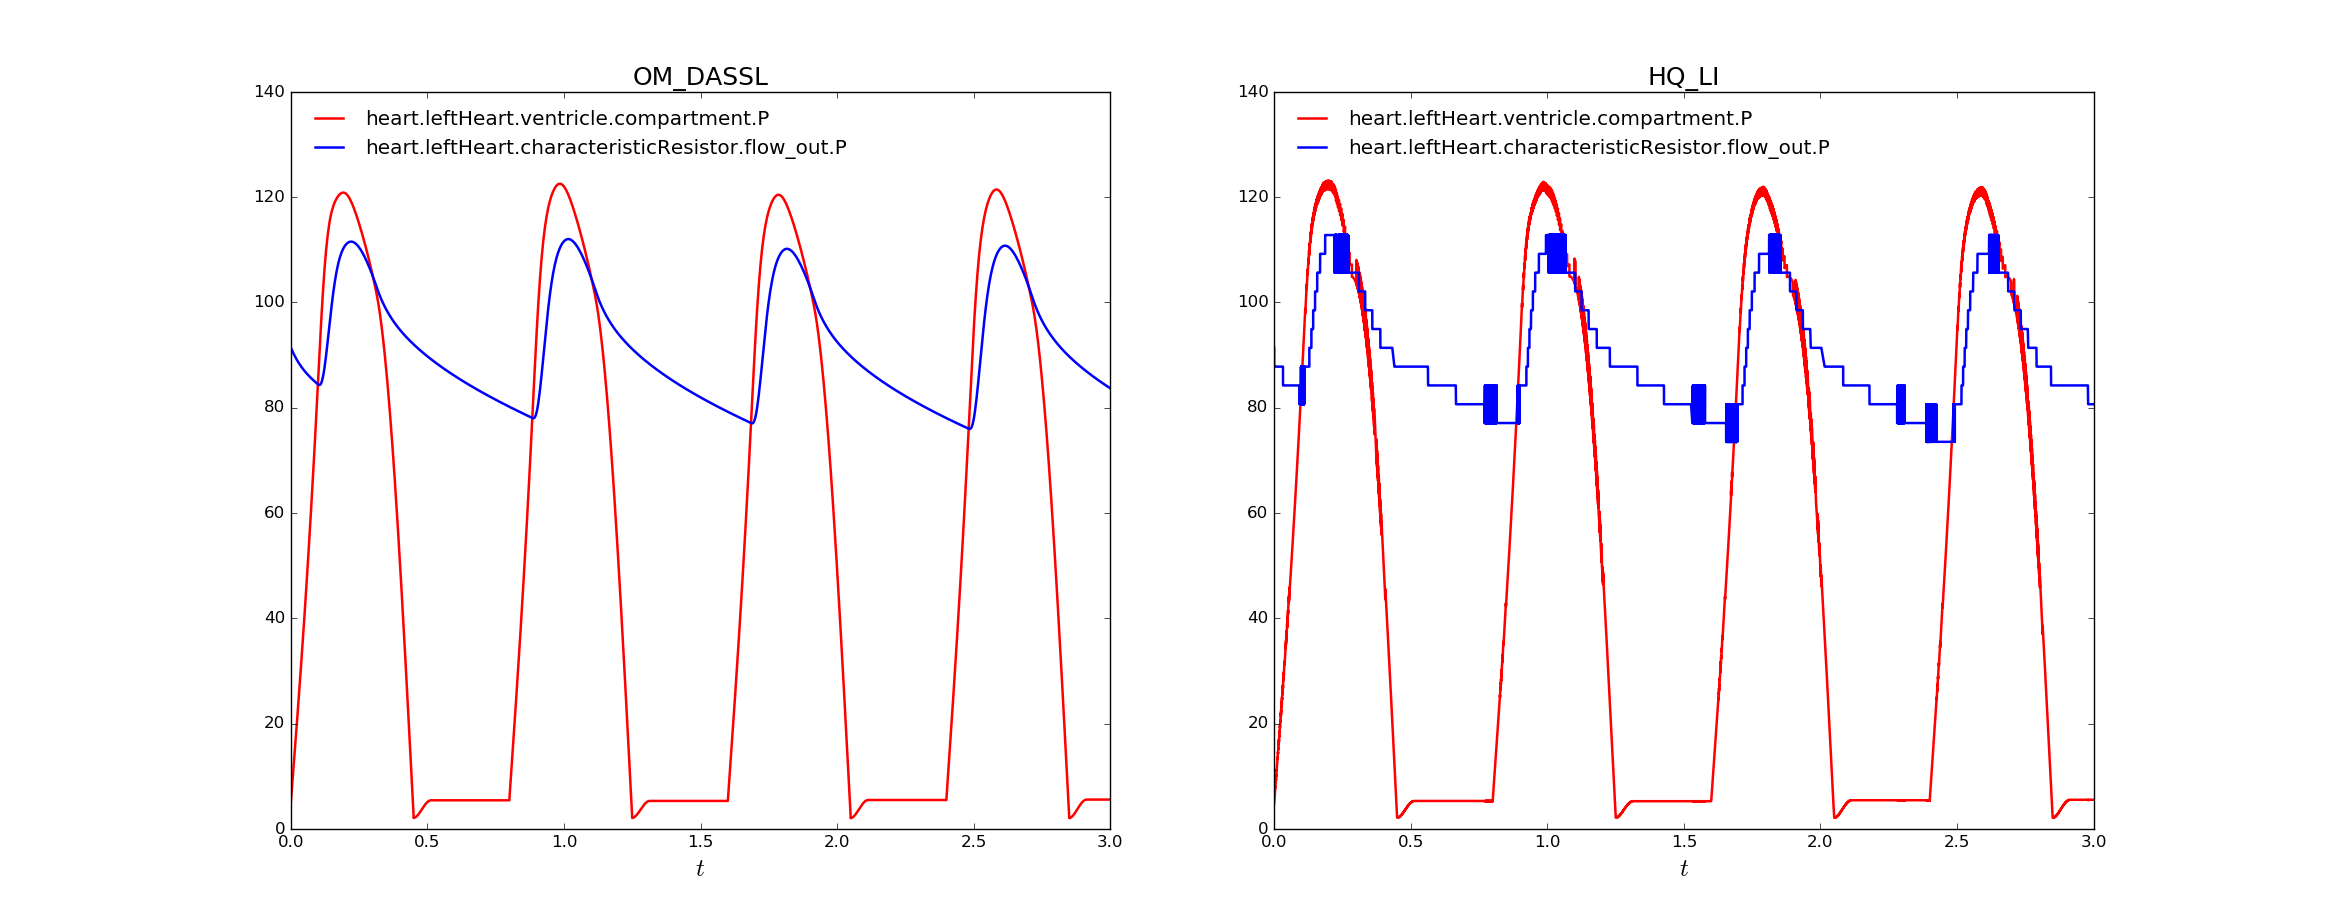
\includegraphics[scale=0.32, clip,trim={50mm 10mm 45mm 10mm}]{./Figures/Model5.png}
\end{center}
\vspace{-0.5cm}
\caption{Simulation results of CardioV for the first 3 seconds of the simulation runs for (a) {\sf{OM\_DASSL}} and (b) {\sf{HQ\_LI}}.}\label{Fig5}
\end{figure}

\newpage

\section{Conclusion}

This document illustrates some of the fundamental differences in simulation results for complex systems using different modeling applications and various solvers within these applications. OpenModelica's DASSL solver is very robust and provides numerically stable results for all the models considered in this document. OpenModelica's QSS solver is computationally very expensive and algorithmically struggles to handle and support event detection and updates. QSS Solver's LIQSS solvers have the ability to solve some models in very short periods of time. The shortcomings with QSS Solver's methods include inaccurate simulation results, incorrect event handling and the fact that the MicroModelica framework must be used, instead of Modelica's environment. HealthQ's QSS solver is outperformed by its LIQSS solver which has concerns related to event handling and slower simulation times but is able to simulate larger, complex models.

The family of QSS Solvers are fundamentally different from traditional solvers ({\em e.g.}\ DASSL, Runge-Kutta and Euler) as they do not discretize the total simulation times. The times at which the ODEs are updated is not known in advance and not all ODEs are necessarily required to be updated at the same time. OpenModelica's framework is created with the aim of discretizing time steps and updating all ODEs simultaneously. This causes considerable inefficiencies with the current QSS methods implemented in OpenModelica. QSS Solver overcomes these obstructions, but the application is still in development and more complex models are often difficult or not possible to convert to the MicroModelica framework. There is thus a need to create an ideal framework to enable the full potential of the QSS solvers.



{\footnotesize
\begin{thebibliography}{10}

\bibitem{ModelicaCC} {\sc Bergero F, Botta M, Campostrini E \& Kofman E}, [Online], Cited 5\textsuperscript{th} April 2016, Available from {\url{http://www.ep.liu.se/ecp/118/048/ecp15118449.pdf}}

\bibitem{micro} {\sc Fern\'andez J \& Kofman E}, {\em $\mu$-Modelica Language Specification}, [Online], Cited 5\textsuperscript{th} April 2016, Available from {\url{http://www.fceia.unr.edu.ar/control/modelica/micromodelicaspec.pdf}}

\bibitem{MigoniKofman2009} {\sc Migoni G \& Fofman E}, 2009, {\em Linearly implicit discrete event methods for stiff ODE's}, Latin American Applied Research, {\bf{39(3)}}, pp.\, 245--254.

\bibitem{OMCompiler} {\sc OMCompiler}, 2016, {\em HealthQ OMCompiler submodule repository}, [Online], Cited 15\textsuperscript{th} March 2016, Available from {\url{https://bitbucket.org/antonpdv/omcompiler}}

\bibitem{OpenModelica} {\sc OpenModelica}, 2016, {\em Open Source Modelica Consortium}, [Online], Cited 15\textsuperscript{th} March 2016, Available from {\url{https://openmodelica.org/}}

\bibitem{DASSL}{\sc Petzold LR}, 1982, {\em A description of DASSL: A differential/algebraic system solver}, Technical Report, Applied Mathematics Division, Sandia National Laboratories, Livermore (CA).

\bibitem{qss}{\sc QSS Solver}, 2016, {\em Modeling and simulation tool for continuous and hybrid systems}, [Online], Cited 15\textsuperscript{th} March 2016, Available from {\url{https://sourceforge.net/projects/qssengine/}}



\end{thebibliography}}


\end{document}